\documentclass[11pt]{article}
\usepackage[margin=1in]{geometry}
\usepackage{amsmath,amssymb}
\usepackage{booktabs}
\usepackage{graphicx}
\usepackage[hidelinks]{hyperref}

\newcommand{\bx}{\mathbf{x}}
\newcommand{\bw}{\mathbf{w}}

\begin{document}

\begin{center}
{\Large\bfseries CSCI3230 / ESTR3108 2026--27 First Term Assignment 2}
\end{center}

\medskip
\noindent\fbox{\begin{minipage}{\dimexpr\linewidth-2\fboxsep-2\fboxrule}
{\itshape I declare that the assignment here submitted is original except for source material explicitly acknowledged, and that the same or closely related material has not been previously submitted for another course. I also acknowledge that I am aware of University policy and regulations on honesty in academic work, and of the disciplinary guidelines and procedures applicable to breaches of such policy and regulations, as contained in the following websites.}

\smallskip
University Guideline on Academic Honesty:\\
\url{http://www.cuhk.edu.hk/policy/academichonesty/}\\
Faculty of Engineering Guidelines to Academic Honesty:\\
\url{http://www.erg.cuhk.edu.hk/erg-intra/upload/documents/ENGG_Discipline.pdf}

\smallskip
Student Name: Jiang Huanyun\\
Student ID: 1155233165
\end{minipage}}

%==================================================================
\section*{Question 1: SVM}

\subsection*{(a) Dual problem, support vectors, hyperplane}

Dual problem:
\[
\max_{\boldsymbol{\alpha}}\ \sum_{i=1}^{8}\alpha_i
-\frac12\sum_{i,j=1}^{8}\alpha_i\alpha_j y_i y_j\,\bx_i^{\top}\bx_j
\qquad\text{s.t.}\quad \sum_{i=1}^{8}\alpha_i y_i=0,\ \alpha_i\ge 0.
\]

Since $\alpha_1=\alpha_8=0.8>0$ (others $0$), by KKT the support vectors are
\textbf{point 1 $(3.5,-2,+1)$ and point 8 $(4,-3.5,-1)$}.

\[
\bw^*=\sum_i \alpha_i y_i \bx_i
=0.8\!\begin{pmatrix}3.5\\-2\end{pmatrix}
-0.8\!\begin{pmatrix}4\\-3.5\end{pmatrix}
=\begin{pmatrix}-0.4\\ 1.2\end{pmatrix},
\]
\[
b^*=y_1-\bw^{*\top}\bx_1=1-\bigl[(-0.4)(3.5)+(1.2)(-2)\bigr]=4.8 .
\]
Optimal hyperplane: \ $\boxed{-0.4x_1+1.2x_2+4.8=0}$.

\subsection*{(b) Test predictions}

Rule: $\hat y=\operatorname{sign}(\bw^{*\top}\bx+b^*)=\operatorname{sign}(-0.4x_1+1.2x_2+4.8)$.

\begin{center}
\begin{tabular}{c|cccccccc}
\toprule
point & 1 & 2 & 3 & 4 & 5 & 6 & 7 & 8\\
\midrule
$f(\bx)$ & 3.2 & 2.8 & 4.8 & 2.6 & $-2.0$ & $-1.0$ & $-4.0$ & $-3.2$\\
$\hat y$ & $+1$ & $+1$ & $+1$ & $+1$ & $-1$ & $-1$ & $-1$ & $-1$\\
\bottomrule
\end{tabular}
\end{center}
All 8 predictions are correct (100\%).

\subsection*{(c) Removing points}

\textbf{Remove point 2} ($\alpha_2=0$, non-support vector): $\bw,b$ unchanged $\Rightarrow$
predictions unchanged.\\
\textbf{Remove point 8} (support vector): the solution changes
($\bw^*\approx(0.235,0.941)^{\top}$, $b^*\approx2.059$), but all test predictions remain the
same (still 100\%).

%==================================================================
\section*{Question 2: Kernel SVM (scikit-learn)}

\begin{itemize}
\item \textbf{Linear kernel, $C=1.0$}: test accuracy $51.02\%$ (matches the example).
\item \textbf{RBF kernel, $C=1.0$, $\gamma=2$}: test accuracy $\mathbf{91.84\%}$ (23 support
vectors) --- exceeds the required 85\%.
\item Also tried: polynomial ($67.3\%$), sigmoid ($46.9\%$).
\end{itemize}

Core code:
\begin{verbatim}
from sklearn.svm import SVC
clf = SVC(kernel='rbf', C=1.0, gamma=2)
clf.fit(X_train, y_train)
acc = clf.score(X_test, y_test)     # 0.9184
\end{verbatim}

Plots (solid line = decision boundary, dashed lines = margins $=\pm1$):

\begin{figure}[h]
\centering
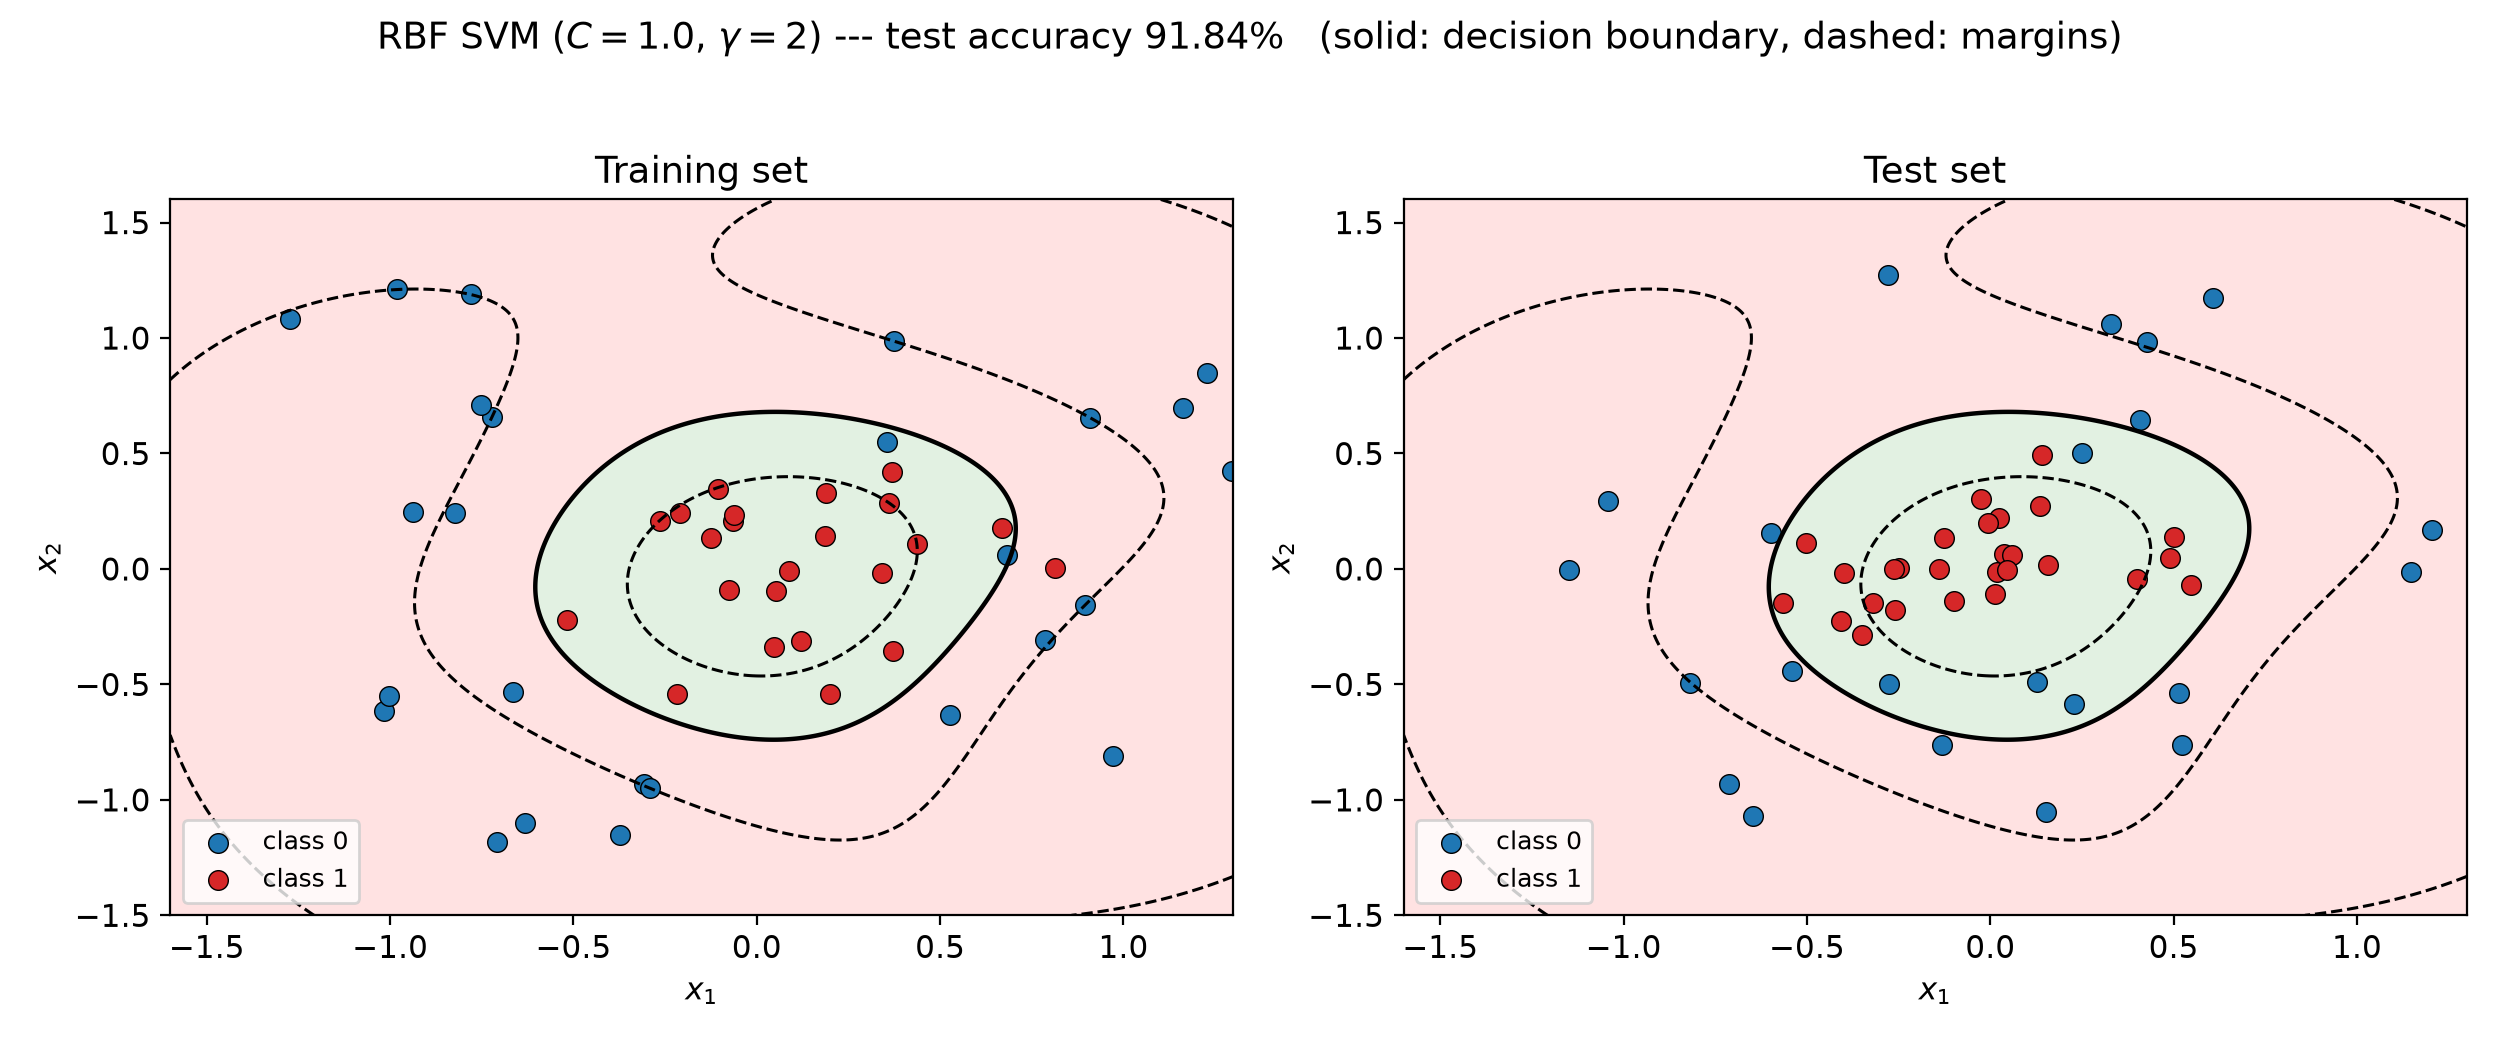
\includegraphics[width=\linewidth]{q2_rbf.png}
\end{figure}

\begin{figure}[h]
\centering
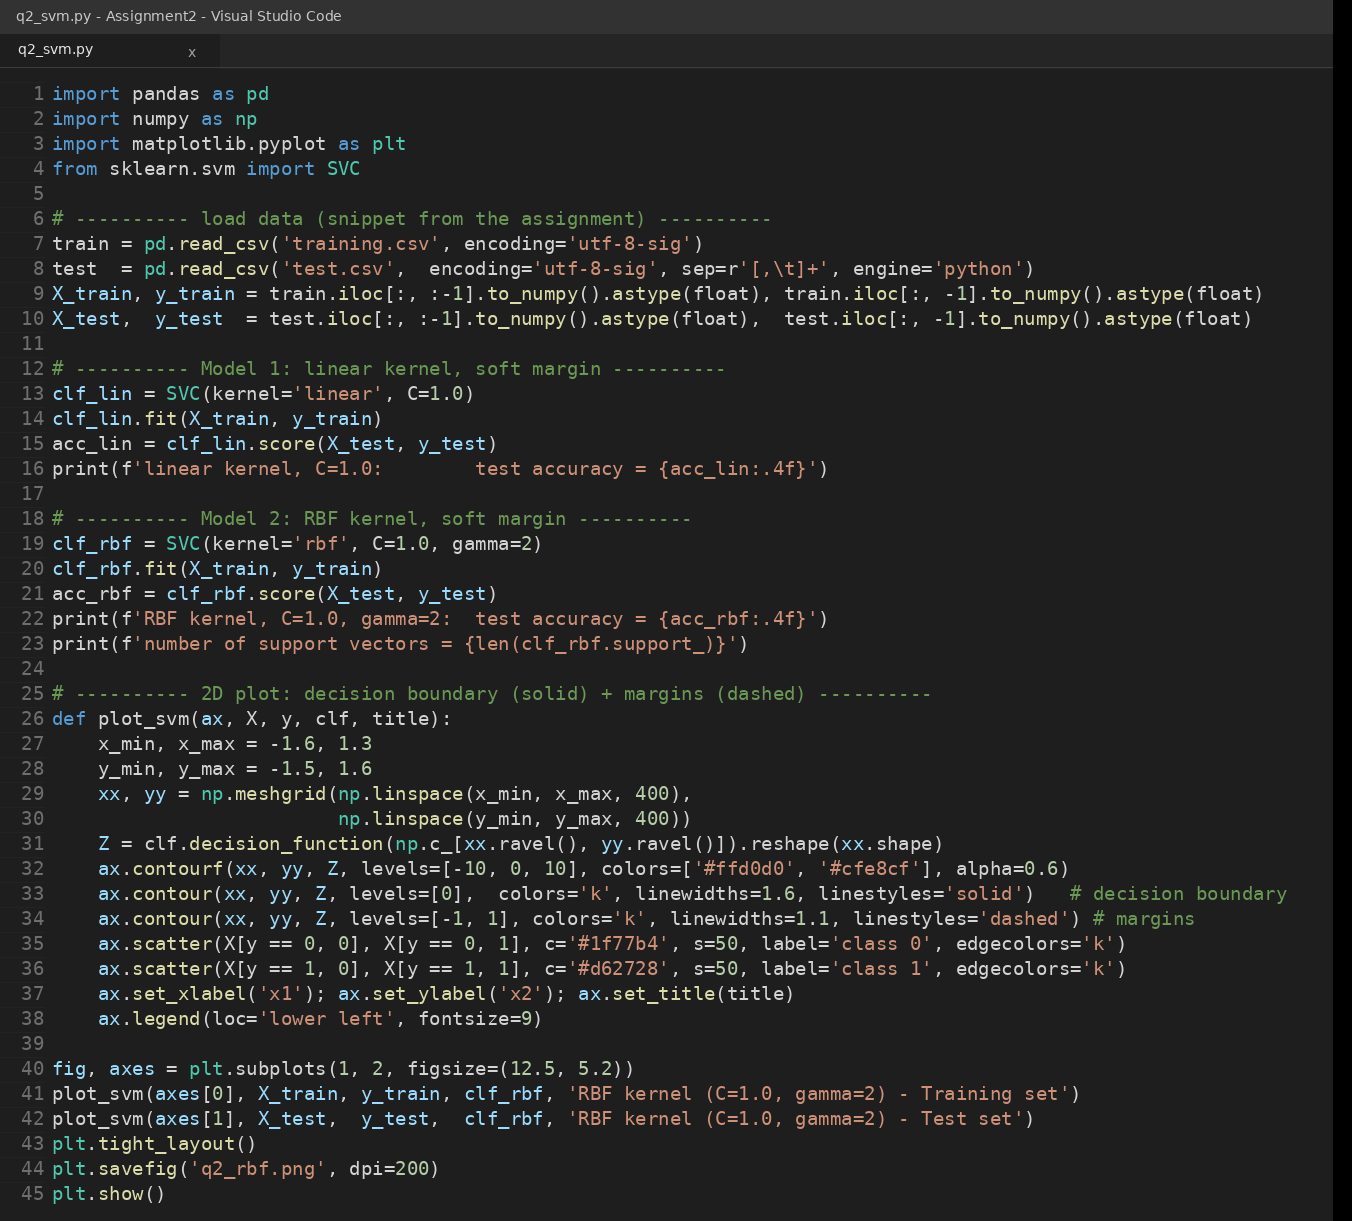
\includegraphics[width=0.72\linewidth]{q2_code_shot.png}
\end{figure}

%==================================================================
\section*{Question 3: K-means and DBSCAN}

Points: $a(1,2)$, $b(2,3)$, $c(2,4)$, $d(6,5)$, $e(3,1)$, $f(3,3)$, $g(4,4)$, $h(7,6)$,
$i(8,8)$, $j(8,9)$, $k(9,4)$, $l(5,9)$, $m(4,7)$, $n(6,8)$, $o(6,4)$.

\subsection*{(a) K-means, first iteration}

Initial centres: $\mu_1=(7,4)$, $\mu_2=(3,6)$, $\mu_3=(7,9)$. Assignment by nearest centre:
$\mu_1:\{d,e,h,k,o\}$,\ \ $\mu_2:\{a,b,c,f,g,m\}$,\ \ $\mu_3:\{i,j,l,n\}$.

Updated centres:
\[
\mu_1^{(1)}=\boxed{(6.2,\ 4)},\qquad
\mu_2^{(1)}=\boxed{(2.67,\ 3.83)},\qquad
\mu_3^{(1)}=\boxed{(6.75,\ 8.5)} .
\]

\subsection*{(b) DBSCAN: $\epsilon=2$, minpts$=3$}

$\epsilon$-neighbourhoods (point itself included):
\begin{center}
\begin{tabular}{clcl}
\toprule
$a$ & $\{a,b\}$ & $i$ & $\{i,j,n\}$\\
$b$ & $\{a,b,c,f\}$ & $j$ & $\{i,j\}$\\
$c$ & $\{b,c,f,g\}$ & $k$ & $\{k\}$\\
$d$ & $\{d,h,o\}$ & $l$ & $\{l,n\}$\\
$e$ & $\{e,f\}$ & $m$ & $\{m\}$\\
$f$ & $\{b,c,e,f,g\}$ & $n$ & $\{i,l,n\}$\\
$g$ & $\{c,f,g,o\}$ & $o$ & $\{d,g,o\}$\\
$h$ & $\{d,h\}$ & &\\
\bottomrule
\end{tabular}
\end{center}

\textbf{Core points} ($|N_\epsilon|\ge3$): $b,c,d,f,g,i,n,o$.\\
\textbf{Border points}: $a,e,h,j,l$.\\
\textbf{Noise points}: $k,m$.

\subsection*{(c) Is $h$ density-reachable from $b$?}

\textbf{Yes}, via the chain \boxed{$b\to c\to g\to o\to d\to h$} (each step from a core point
to a point in its $\epsilon$-neighbourhood).

\subsection*{(d) Clusters}

Cluster 1: $\{a,b,c,d,e,f,g,h,o\}$;\quad Cluster 2: $\{i,j,l,n\}$;\quad Noise: $k,m$.

%==================================================================
\section*{Question 4: Hierarchical clustering (group average)}

\begin{center}
\begin{tabular}{c|ccccc}
\toprule
& A & B & C & D & E\\
\midrule
A & 0 & 8 & 6 & 2 & 1\\
B & 8 & 0 & 7 & 3 & 6\\
C & 6 & 7 & 0 & 9 & 5\\
D & 2 & 3 & 9 & 0 & 4\\
E & 1 & 6 & 5 & 4 & 0\\
\bottomrule
\end{tabular}
\end{center}

Group average: $d(U,V)=\frac{1}{|U||V|}\sum_{u\in U}\sum_{v\in V}d(u,v)$.

\textbf{Step 1.} $d(A,E)=1$ min $\Rightarrow$ merge into $AE$.\\
Updated: $AE\text{--}B=7$, $AE\text{--}C=5.5$, $AE\text{--}D=3$.

\textbf{Step 2.} $d(B,D)=3$ min $\Rightarrow$ merge into $BD$.\\
$d(AE,BD)=\frac{8+6+2+4}{4}=5$, \ $d(C,BD)=\frac{7+9}{2}=8$.

\textbf{Step 3.} $d(AE,BD)=5$ min $\Rightarrow$ merge into $AEBD$.\\
$d(C,AEBD)=\frac{6+5+7+9}{4}=6.75$.

\textbf{Step 4.} All merged at distance $6.75$.

Merge order: \boxed{(A,E)\!\xrightarrow{1}\!(B,D)\!\xrightarrow{3}\!(AE,BD)\!\xrightarrow{5}\!(AEBD,C)\!\xrightarrow{6.75}}

\begin{figure}[h]
\centering
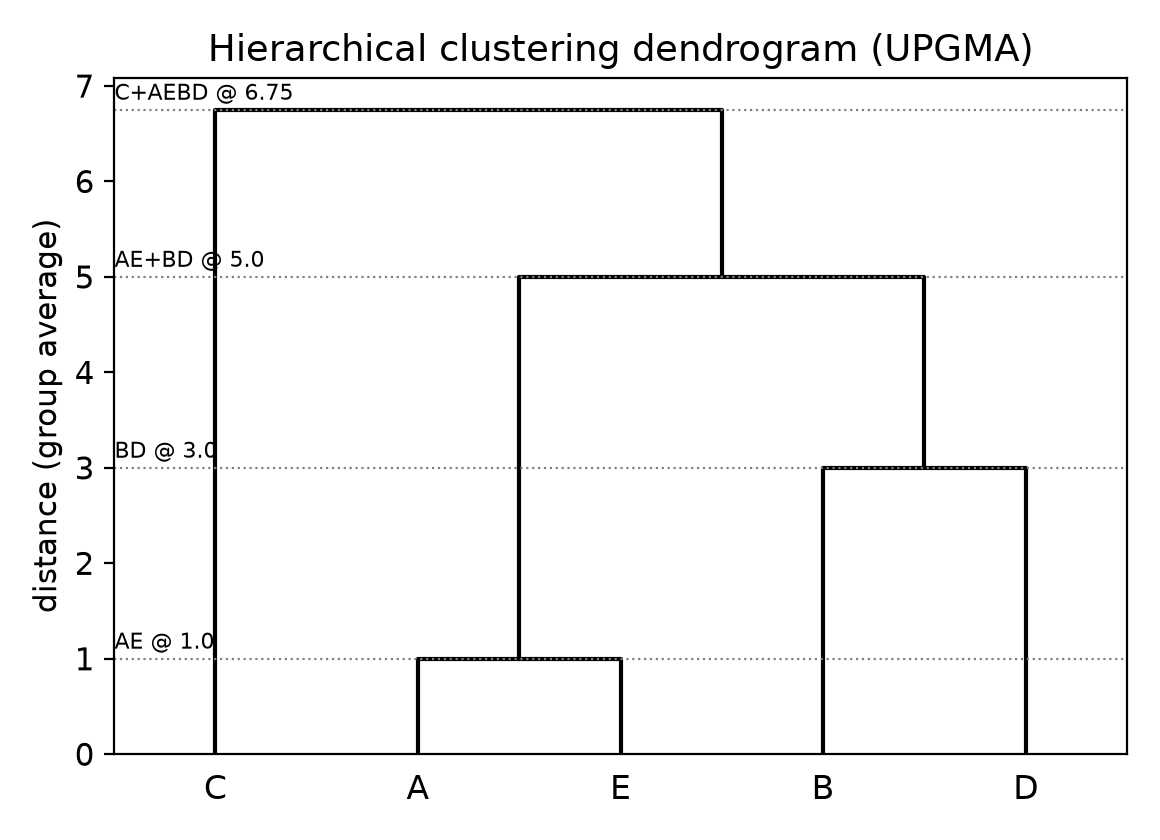
\includegraphics[width=0.75\linewidth]{q4_dendrogram.png}
\end{figure}

\end{document}
